\chapter{Discussion}\label{chap:discussion}

We discuss our formalisation. Finally a conclusion.


\section{Convergence of Rewrite Sequences}\label{sec:convergence}

The inductively defined rewrite sequences from Section~\ref{sec:seq}
are not necessarily (weakly) convergent. A rewrite sequence of limit
length satisfies the condition that the target terms of the
\coqref{Rewriting.Lim}{\coqdocconstructor{Lim}} branches converge but
this is obviously too weak to establish convergence of the rewrite
sequence itself.

The depths of the rewrite steps are not considered at all in our
formalisation and therefore it obviously does not implement strong
convergence. Furthermore, the discussion in this section also applies
to the notions of continuity.

We consider an example of a rewrite sequence that satisfies the
inductive definition but is not weakly convergent. Let $A$ be a
constant and $B, C, D$ unary function symbols. We use the following
three rewrite rules:
\begin{align*}
  \rho_1 \, : \, A \to B(A) \qquad \qquad
  \rho_2 \, : \, C(x) \to D(x) \qquad \qquad
  \rho_3 \, : \, D(x) \to C(x)
\end{align*}
The term $C(A)$ rewrites in $\omega$ many $\rho_1$-steps to
$C(B^\omega)$.
\begin{center}
{\footnotesize\begin{tikzpicture}[node distance=50pt]
\tikzstyle{level}=[level distance=20pt,sibling distance=22pt]
\node (a) {$C$} child { node {$A$} };
\node (b) [right of=a] {$C$} child { node {$B$} child { node {$A$} } };
\node (c) [right of=b] {$C$} child { node {$B$} child { node {$B$}
    child { node {$A$} } } };
\node (d) [right of=c,node distance=80pt] {$C$} child { node {$B$}
  child { node {$B$} child { node {$B$} child { node[below=-6pt]
        {\scriptsize$\vdots$} } } } };
\path (a) -- (b) node[midway,below=-1pt] {$\rightarrow_{\rho_1}$};
\path (b) -- (c) node[midway,below=-1pt] {$\rightarrow_{\rho_1}$};
\path (c) -- (d) node[midway,below=-1pt] {$\rightarrow_{\rho_1} \quad \cdots$};
\end{tikzpicture}}
\end{center}\vspace{-0.8\baselineskip}
We modify this rewrite sequence such that in between every two
$\rho_1$-steps, the root symbol $C$ is changed to $D$ and back to
$C$. The resulting rewrite sequence does not have a limit and is not
weakly convergent.
\begin{center}
{\footnotesize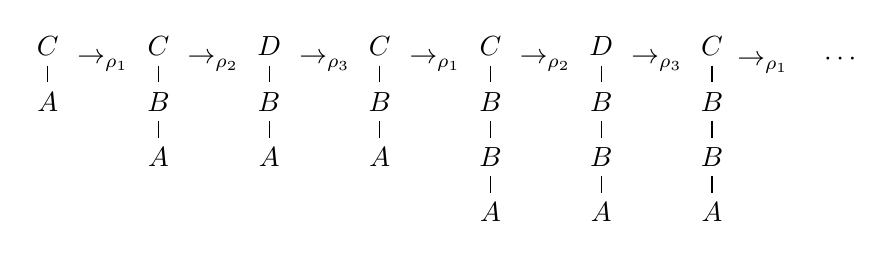
\begin{tikzpicture}[node distance=40pt]
\tikzstyle{level}=[level distance=20pt,sibling distance=22pt]
\node (a) {$C$} child { node {$A$} };
\node (a') [right of=a] {$C$} child { node {$B$} child { node {$A$} } };
\node (a'') [right of=a'] {$D$} child { node {$B$} child { node {$A$} } };
\node (b) [right of=a''] {$C$} child { node {$B$} child { node {$A$} } };
\node (b') [right of=b] {$C$} child { node {$B$} child { node {$B$}
    child { node {$A$} } } };
\node (b'') [right of=b'] {$D$} child { node {$B$} child { node {$B$}
    child { node {$A$} } } };
\node (c) [right of=b''] {$C$} child { node {$B$} child { node {$B$}
    child { node {$A$} } } };
\node (d) [right of=c] {};
\path (a) -- (a') node[midway,below=-1pt] {$\rightarrow_{\rho_1}$};
\path (a') -- (a'') node[midway,below=-1pt] {$\rightarrow_{\rho_2}$};
\path (a'') -- (b) node[midway,below=-1pt] {$\rightarrow_{\rho_3}$};
\path (b) -- (b') node[midway,below=-1pt] {$\rightarrow_{\rho_1}$};
\path (b') -- (b'') node[midway,below=-1pt] {$\rightarrow_{\rho_2}$};
\path (b'') -- (c) node[midway,below=-1pt] {$\rightarrow_{\rho_3}$};
\path (c) -- (d) node[pos=.8,below=-1pt] {$\rightarrow_{\rho_1} \quad \cdots$};
\end{tikzpicture}}
\end{center}\vspace{-0.8\baselineskip}
We can define this rewrite sequence as the limit of
$(\varphi_n)_{n \in \mathbb{N}}$, where $\concat$ denotes
concatenation of rewrite sequences:
\begin{align*}
  \varphi_0 \, &: \, \mbox{\emph{empty}}\\ % TODO: or C(A) \to^0 C(A)
  \varphi_{n + 1} \, &: \, \varphi_n \concat C(B^n(A)) \to_{\rho_1}
  C(B^{n + 1}(A)) \to_{\rho_2} D(B^{n + 1}(A)) \to_{\rho_3} C(B^{n +
    1}(A))
\end{align*}
The target terms $C(B^{n + 1}(A))$ converge to $C(B^\omega)$ and this
construction can thus be used with our inductive definition of rewrite
sequences, where we take $\varphi_n$ to be the $n$\textsuperscript{th}
branch of the \coqref{Rewriting.Lim}{\coqdocconstructor{Lim}}
constructor.

% $\varphi_n$ is the prefix of length $3n$.

% 'stuttering convergence'
% convergence with hiccups
% the difference between t_n and the limit t is oscillating

It is not clear to us whether there is some natural translation of the
convergence conditions to our formalisation.
%Without such a translation, we feel our definitions are not
%satisfactory.
For completeness we include a (not so natural) translation of
convergence, but we were not able to use it in our development. Even
proving the simplest convergent rewrite sequences to satisfy these
definitions seems too involved.
\begin{singlespace}
\begin{coqdoccode}
\coqdocnoindent
\coqdockw{Fixpoint}
\coqdef{Rewriting.weaklyconvergent}{weakly\_convergent}{\coqdocdefinition{weakly\_convergent}}
\coqdocvar{s} \coqdocvar{t} (\coqdocvar{$\varphi$} : \coqdocvar{s}
\coqref{Rewriting.sequence}{$\rewrites_\mathcal{R}$} \coqdocvar{t}) :
\coqdockw{Prop}
:=\coqdoceol
\coqdocindent{1.00em}
\coqdockw{match} \coqdocvariable{$\varphi$} \coqdockw{with}\coqdoceol
\coqdocindent{1.00em}
\ensuremath{|} \coqref{Rewriting.Nil}{\coqdocconstructor{Nil}}
\coqdocvar{\_}          \ensuremath{\Rightarrow}
\coqexternalref{http://coq.inria.fr/stdlib/Coq.Init.Logic}{True}{\coqdocinductive{True}}\coqdoceol
\coqdocindent{1.00em}
\ensuremath{|} \coqref{Rewriting.Cons}{\coqdocconstructor{Cons}}
\coqdocvar{\_} \coqdocvar{\_} \coqdocvar{$\psi$} \coqdocvar{\_}
\coqdocvar{\_} \ensuremath{\Rightarrow}
\coqref{Rewriting.weaklyconvergent}{\coqdocdefinition{weakly\_convergent}}
\coqdocvariable{$\psi$}\coqdoceol
\coqdocindent{1.00em}
\ensuremath{|} \coqref{Rewriting.Lim}{\coqdocconstructor{Lim}}
\coqdocvar{\_} \coqdocvar{\_} \coqdocvar{f} \coqdocvar{t}
\coqdocvar{\_}  \ensuremath{\Rightarrow}
(\ensuremath{\forall} \coqdocvar{n},
\coqref{Rewriting.weaklyconvergent}{\coqdocdefinition{weakly\_convergent}}
(\coqdocvariable{f} \coqdocvariable{n})) \ensuremath{\land}\coqdoceol
\coqdocindent{2.00em}
\ensuremath{\forall} \coqdocvar{d}, \ensuremath{\exists}
\coqdocvar{$\iota$}, \ensuremath{\forall} \coqdocvar{$\kappa$},\coqdoceol
\coqdocindent{3.00em}
\coqdocvariable{$\varphi$}[\coqdocvariable{$\iota$}]$^\textsc{seq}$ \coqref{Rewriting.embed}{$\sqsubseteq$}
\coqdocvariable{$\varphi$}[\coqdocvariable{$\kappa$}]$^\textsc{seq}$
\ensuremath{\rightarrow}
\coqdocvariable{$\varphi$}[\coqdocvariable{$\kappa$}]$^\textsc{l}$
\coqref{TermEquality.termequpto}{\equpto{\coqdocvariable{d}}}
\coqdocvariable{t}\coqdoceol
\coqdocindent{1.00em}
\coqdockw{end}.\coqdoceol
\coqdocemptyline
\coqdocnoindent
\coqdockw{Fixpoint}
\coqdef{Rewriting.stronglyconvergent}{strongly\_convergent}{\coqdocdefinition{strongly\_convergent}}
\coqdocvar{s} \coqdocvar{t} (\coqdocvar{$\varphi$} : \coqdocvar{s} \coqref{Rewriting.sequence}{$\rewrites_\mathcal{R}$} \coqdocvar{t}) : \coqdockw{Prop}
:=\coqdoceol
\coqdocindent{1.00em}
\coqdockw{match} \coqdocvariable{$\varphi$} \coqdockw{with}\coqdoceol
\coqdocindent{1.00em}
\ensuremath{|} \coqref{Rewriting.Nil}{\coqdocconstructor{Nil}}
\coqdocvar{\_}          \ensuremath{\Rightarrow}
\coqexternalref{http://coq.inria.fr/stdlib/Coq.Init.Logic}{True}{\coqdocinductive{True}}\coqdoceol
\coqdocindent{1.00em}
\ensuremath{|} \coqref{Rewriting.Cons}{\coqdocconstructor{Cons}}
\coqdocvar{\_} \coqdocvar{\_} \coqdocvar{$\psi$} \coqdocvar{\_}
\coqdocvar{\_} \ensuremath{\Rightarrow}
\coqref{Rewriting.stronglyconvergent}{\coqdocdefinition{strongly\_convergent}}
\coqdocvariable{$\psi$}\coqdoceol
\coqdocindent{1.00em}
\ensuremath{|} \coqref{Rewriting.Lim}{\coqdocconstructor{Lim}}
\coqdocvar{\_} \coqdocvar{\_} \coqdocvar{f} \coqdocvar{t}
\coqdocvar{\_}  \ensuremath{\Rightarrow}
(\ensuremath{\forall} \coqdocvar{n},
\coqref{Rewriting.stronglyconvergent}{\coqdocdefinition{strongly\_convergent}}
(\coqdocvariable{f} \coqdocvariable{n})) \ensuremath{\land}\coqdoceol
\coqdocindent{2.00em}
\ensuremath{\forall} \coqdocvar{d}, \ensuremath{\exists}
\coqdocvar{$\iota$}, \ensuremath{\forall} \coqdocvar{$\kappa$},\coqdoceol
\coqdocindent{3.00em}
\coqdocvariable{$\varphi$}[\coqdocvariable{$\iota$}]$^\textsc{seq}$
\coqref{Rewriting.embed}{$\sqsubseteq$}
\coqdocvariable{$\varphi$}[\coqdocvariable{$\kappa$}]$^\textsc{seq}$
\ensuremath{\rightarrow}
\coqdocvariable{d} $\le$
\coqdocdefinition{depth}
\coqdocvariable{$\varphi$}[\coqdocvariable{$\kappa$}]$^\textsc{stp}$\coqdoceol
\coqdocindent{1.00em}
\coqdockw{end}.\coqdoceol
\end{coqdoccode}
\end{singlespace}
Here it should be possible to prove that
\coqref{Rewriting.stronglyconvergent}{\coqdocdefinition{strongly\_convergent}}
implies
\coqref{Rewriting.weaklyconvergent}{\coqdocdefinition{weakly\_convergent}}.


\section{Representing Rewrite Sequences}

% TODO: leave out ', with the appropriate conditions...' ?
In Definition~\ref{def:seq}, transfinite rewrite sequences are
introduced as partial functions from ordinals to rewrite steps, with
the appropriate conditions on source and target terms of subsequent
rewrite steps. Could we not translate this directly to \Coq?

% TODO: one problem, and other problem?
A problem is that we would need a decidable order on the
ordinals.\footnote{Consider a non-trivial rewrite sequence of length
  $\lambda$. For every ordinal $\alpha < \lambda$, the partial
  function representing this rewrite sequence must decide what step to
  produce.}
The order on our tree ordinals is not decidable. This could be
remedied by using a different representation for the ordinals, for
example axiomatically, as Cantor normal forms, or as sets. We feel
that the inductively defined tree ordinals are a more natural
representation in the constructive type theory of \Coq.

Comparison of ordinals up to some given upper bound may be decidable,
so another remedy for this problem would be to only consider rewrite
sequences of limited length. Motivated by the Compression Lemma, we
could go even further and restrict our representation to rewrite
sequences of length $\le \omega$. This would severely cripple our
formalisation, since much of the theory of infinitary rewriting could
not be developed with this representation (e.g. the Compression Lemma
itself). % and many compressed rewrite sequences are unnatural

Another argument in favour of our representation based on tree
ordinals is that it seems natural for a \Coq formalisation. As a
comparison, lists of finite length are usually defined by induction in
\Coq, not as partial functions from the natural numbers. Our
representation can be seen as a generalisation of inductively defined
finite lists to lists of transfinite length.


\section{Design Choices}

We describe a number of design choices for our formalisation.

%One-hole contexts vs multi-hole contexts (possible using extended signature).

%Casteran's ordinals in Veblen nf vs Mamane's set-theoretic ordinals vs tree
%ordinals.

%Bisimilarity in steps.

%The embedding relation and order on ordinals by Hancock, are there other
%choices?

%Positions are just lists (using option types) versus a safe position
%type parameterised by a term.

%Coinductive terms versus functions from lists of positions.

%Why \Coq?


\section{Conclusion}

Our representation feels natural, but the traditional convergence
definitions do not fit (easily). Maybe there are alternatives to our
embedding relation, or can we index the steps in a different way than
with predecessor indices.

Functions from ordinals to steps have other problems. They could be
investigated, especially using other ordinal representations such as
cantor normal form. But this is very not \Coq-like (partial functions
and algebraic representations). See also recent work by Ketema.

TODO: additional remarks on productivity and guardedness restriction?
There has been a lot of work in termination of recursive definitions.

Representation is original.

Original goal was compression.

%It is not clear to us whether there is some natural translation of the
%convergence conditions to our formalisation.
Without such a translation, we feel our definitions are not
satisfactory.
